\documentclass{standalone}
\usepackage{tikz}
\usetikzlibrary{arrows.meta}

\begin{document}
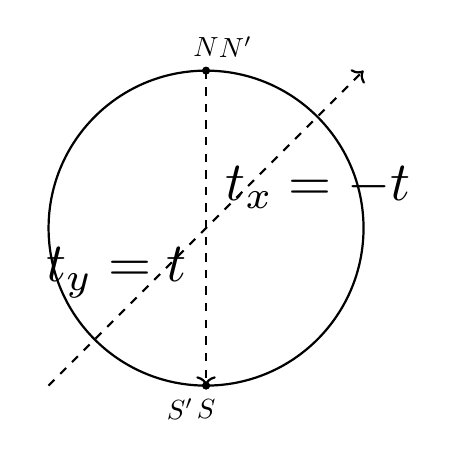
\begin{tikzpicture}[scale=2]

% Draw the spatial sphere
\draw[thick] (0,0) circle (1);

% Mark the poles
\node[circle, fill, inner sep=1pt, label=above:$N$] at (0,1) {};
\node[circle, fill, inner sep=1pt, label=below:$S$] at (0,-1) {};

% Draw the geodesic (if applicable)
\draw[dashed, thick, ->] (-1,-1) -- (1,1); % Geodesic from N to S

% Apply the de Sitter time-translation transformation
\node[circle, fill, inner sep=1pt, label=above right:$N'$] at (0,1) {};
\node[circle, fill, inner sep=1pt, label=below left:$S'$] at (0,-1) {};

% Draw the geodesic after transformation
\draw[dashed, thick, ->] (0,1) -- (0,-1); % Geodesic along the z-axis

% Label the transformation
\node[midway, above right] at (0.5, 0.5) {$t_x = -t$};
\node[midway, below left] at (-0.5, -0.5) {$t_y = t$};

\end{tikzpicture}
\end{document}